\chapter{Propuesta}\label{chapter:proposal}

En este cap\'itulo se propone primeramente un nuevo modelo no lineal. Posteriormente se describe el m\'odulo implementado, el cual contiene todos estos modelos no lineales, m\'etricas y algoritmos.

\section{Modelo PPSLIP}

En la tabla 2.1 se muestra una peque\~na comparaci\'on entre los modelos LIP y PSLIP, en cuanto a la suma. En el modelo LIP se asume que ya el p\'ixel representa un tono de gris.

\begin{table}
	\caption{Comparativa de la suma en los modelos LIP y PSLIP}
	\begin{center}
		\begin{tabular}{|l|l|}
			\hline 
			\textbf{LIP} & \textbf{PSLIP}\\
			\hline
			$45 \boxplus 15 = 57.36$ & $45 \oplus 15 = 55.29$\\
			\hline
			$45 \boxplus 70 = 102.69$ & $45 \oplus 15 = 94.95$\\
			\hline
			$45 \boxplus 15 = 168.63$ & $45 \oplus 15 = 158.60$\\
			\hline
			$45 \boxplus 15 = 222.20$ & $45 \oplus 15 = 216.35$\\
			\hline
		\end{tabular}
	\end{center}
\end{table}

Como se puede apreciar en los ejemplos de la tabla 2.1 al ejercer la suma se pierde m\'as informaci\'on en el modelo PSLIP que en el modelo LIP. Por ende si para evitar la p\'erdida de informaci\'on en el modelo LIP se presenta un nuevo modelo parametrizado, tiene gran sentido parametrizar tambi\'en el modelo PSLIP para lograr este fin. Por eso como parte de este trabajo se presenta el Modelo Pseudo-logar\'imico Parametrizado para el Procesamiento de Im\'agenes (PPSLIP). Para lograr esto lo que se hizo fue parametrizar la funci\'on de cambio de nivel de gris $u$ a tono de gris $v$ y su inversa de la siguiente forma:

\begin{equation}
	v=\frac{u}{\delta(M)}
\end{equation}

\begin{equation}
	u=\delta(M)v
\end{equation}

tal que $\delta(M) \geq M$.

Es sencillo comprobar que a medida que $\delta(M)\to\ +\infty$ las operaciones aritm\'eticas se asemejan a las operaciones aritm\'eticas lineales. Por ejemplo, sustituyendo (2.1) en (1.27) y luego sustituyendo esto en (2.2) se tiene que la suma de dos niveles de grises es:

\begin{equation}
	u_1\oplus u_2=\delta(M)\frac{\frac{u_1}{\delta(M)}+\frac{u_2}{\delta(M)}-2\left(\frac{u_1}{\delta(M)}\cdot\frac{u_2}{\delta(M)}\right)}{1-\frac{u_1}{\delta(M)}\cdot\frac{u_2}{\delta(M)}}
\end{equation}

Calculando el l\'imite de (2.3) cuando $\delta(M)\to\ +\infty$ se tiene que:

\begin{center}
	$\displaystyle\lim_{\delta(M) \to +\infty}\delta(M)\frac{\frac{u_1}{\delta(M)}+\frac{u_2}{\delta(M)}-2\frac{u_1}{\delta(M)}\cdot\frac{u_2}{\delta(M)}}{1-\frac{u_1}{\delta(M)}\cdot\frac{u_2}{\delta(M)}}$
	
	$\displaystyle=\lim_{\delta(M) \to +\infty}\frac{u_1+u_2-2\frac{u_1u_2}{\delta(M)}}{1-\frac{u_1u_2}{\delta(M)^2}}$
	
	$\displaystyle=\lim_{\delta(M) \to +\infty}\frac{u_1+u_2-2\frac{u_1u_2}{\delta(M)}\nearrow^0}{1-\frac{u_1u_2}{\delta(M)^2}\nearrow^0}$
	
	$\displaystyle=\frac{u_1+u_2}{1}$
	
	$\displaystyle=u_1+u_2$
\end{center}

De manera similar se puede proceder para con la multiplicaci\'on escalar y la resta.

Obs\'ervese que al parametrizar solo la funci\'on de cambio de nivel a tono de gris se parametrizan todas las operaciones con el mismo par\'ametro. Una forma de parametrizar las operaciones de forma independiente es eliminar las funciones de cambio y hacer los cambios directamente en las operaciones como se hizo para el c\'alculo de l\'imite anterior. Esta variante fue la que se sigui\'o en la implementaci\'on del modelo, por lo tanto ya no se utilizan las funciones de cambio y la adici\'on queda definida como:

\begin{equation}
	u_1\oplus u_2=\frac{u_1+u_2-\frac{2u_1u_2}{\gamma(M)}}{1-\frac{u_1u_2}{\gamma(M)^2}}
\end{equation}

Mientras que la multiplicaci\'on por un escalar no negativo $c\in\mathbb{R}^+$ se define como:

\begin{equation}
	c\otimes u=\frac{cu}{1+\frac{(c-1)u}{\gamma(M)}}
\end{equation}

y la resta para un par de p\'ixeles $u_1,u_2:u_1\geq u_2$ es:

\begin{equation}
	u_1\ominus u_2=\frac{u_1-u_2}{1+\frac{u_1u_2}{k(M)^2}-\frac{2u_2}{k(M)}}
\end{equation}

Las funci\'on fundamental del isomorfismo se define como:

\begin{equation}
	\varphi(u)=\frac{u}{\lambda(M)-u}
\end{equation}

y su inversa:

\begin{equation}
	\varphi^{-1}(x)=\lambda(M)\frac{x}{1+x}
\end{equation}

\section{M\'odulo de Python de Modelos no Lineales para el Procesamiento de Im\'agenes}

El m\'odulo implementado cuenta con dos tipos de objetos fundamentales: las estructuras y los espacios.

\subsection{Estructuras}

\begin{figure}
	\begin{center}
		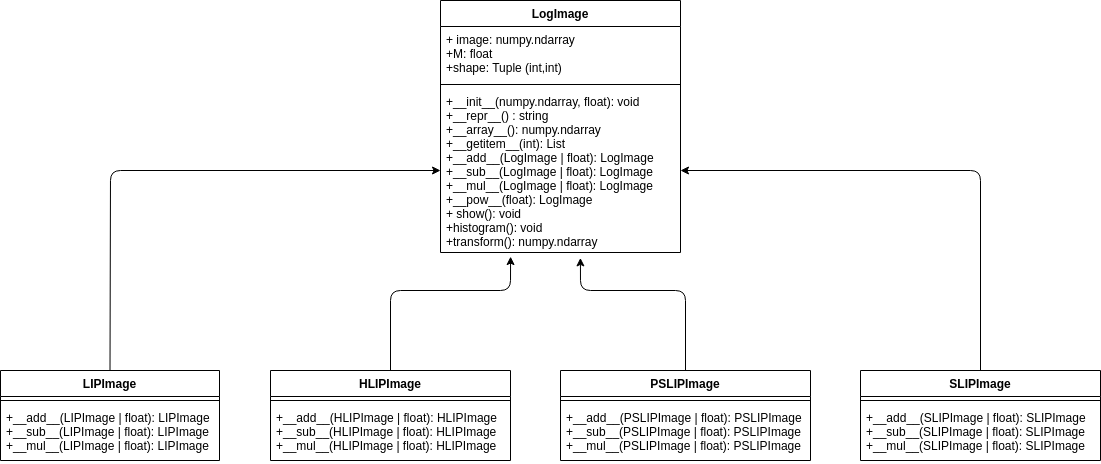
\includegraphics[width=16.0 cm]{images/structures_class_diagram.png}
		\caption{Diagrama de clases de las estructuras no lineales}
	\end{center}
\end{figure}

Para entender mejor la composici\'on del m\'odulo v\'ease el diagrama de clases de la Figura 2.1. Como se puede ver en esta figura se tiene una clase abstracta \verb|LogImage| de la cual heredan las clases \verb|LIPImage|, \verb|HLIPImage|, \verb|PSLIPImage| y \verb|SLIPImage|. Cada una de estas clases representa una imagen en los respectivos modelos: LIP, HLIP, PSLIP y SLIP. Los atributos de la clase padre son:

\begin{itemize}
	\item \verb|M|: el valor de $M$ tal que los niveles de gris de los p\'ixeles de la imagen original se encuentran en el rango $[0,M)$.
	\item \verb|image|: la imagen transformada al espacio de la estructura.
	\item \verb|shape|: una \textit{tupla} de dos enteros que son las dimensiones de la imagen.
\end{itemize}

Adem\'as se definieron los siguientes m\'etodos:

\begin{itemize}
	\item \verb|__init__|: El constructor, que recibe como par\'ametros la imagen original y el valor de $M$ correspondiente. Esta funci\'on en cada una de las diferentes clases transforma la imagen en el espacio original al espacio de la estructura, aplicando primeramente la funci\'on de cambio a tono de gris y luego la funci\'on del isomorfismo.
	\item \verb|__repr__|: Para representar una instancia como un \textit{string} semejante a su atributo \verb|image|.
	\item \verb|__array__|: Que permite que la instancia pueda ser utilizada como un \verb|numpy.ndarray| por las funciones de la librer\'ia \verb|numpy| utilizando su atributo \verb|image|.
	\item \verb|__getitem__|: Que permite indexar una instancia con un entero positivo \verb|i| devolviendo la fila $i$ de la imagen, la cual puede indexarse para acceder a un p\'ixel en espec\'ifico.
	\item \verb|__add__|, \verb|__sub__| y \verb|__mul__|: Que redefinen los operadores \verb|+|, \verb|-| y \verb|*| para la suma, resta y multiplicaci\'on respectivamente. Obs\'ervese que cada una de las clases que heredan de \verb|LogImage| redefinen estos operadores admitiendo solamente para realizar la operaci\'on una instancia de la misma clase, un entero o un n\'umero flotante, dando como salida una nueva instancia de la clase resultado de la operaci\'on realizada. Aclarar que la multiplicaci\'on de dos im\'agenes se hace por parejas de p\'ixeles en la misma posici\'on, diferente a la multiplicaci\'on cl\'asica de matrices.
	\item \verb|__pow__|: Que redefine el operador \verb|**| para elevar la imagen a un escalar $\lambda\in \mathbb{R}$.
	\item \verb|show|: Que lo que hace es mostrar como se ve la imagen en dicho espacio.
	\item \verb|histogram|: Que muestra el histograma de la imagen en dicho espacio.
	\item \verb|transform|: Transforma la imagen al espacio original aplicando la inversa de la funci\'on del isomorfismo y posteriormente la funci\'on de cambio a niveles de grises.
\end{itemize}

Con las clases vistas anteriormente se puede transformar una imagen a otra imagen en el espacio deseado, operar con ella en dicho espacio y luego el resultado regresarlo al espacio original. Obs\'ervese que los espacios parametrizados no se implementaron con estas estructuras, pues estos utilizan diferentes par\'ametros para las diferentes operaciones, algo que no se puede hacer utilizando las estructuras pues una imagen solo se puede transformar de un espacio a otro con un \'unico valor de $M$.

\subsection{Espacios}

\begin{figure}
	\begin{center}
		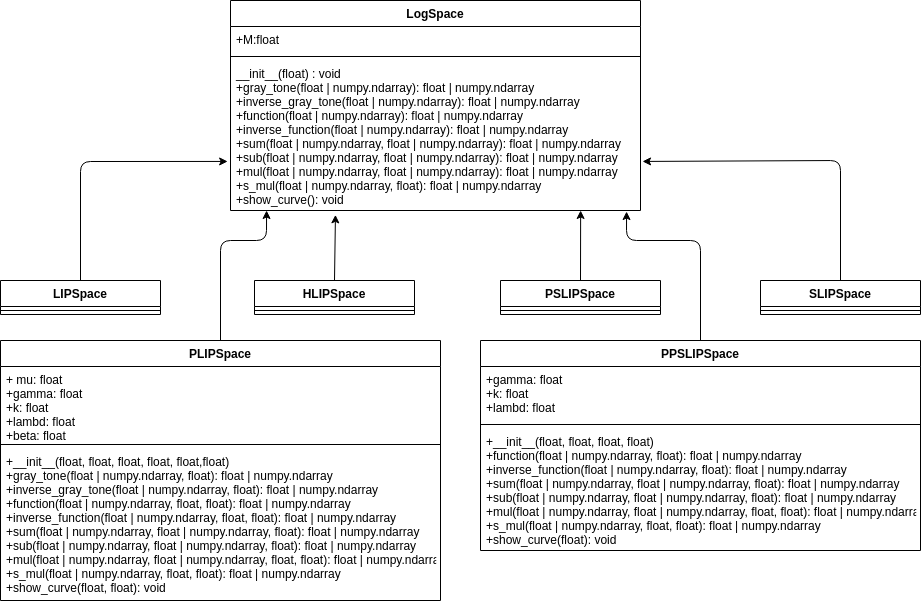
\includegraphics[width=16.0 cm]{images/spaces_class_diagram.png}
		\caption{Diagrama de clases de los espacios no lineales}
	\end{center}
\end{figure}

Para entender mejor la composici\'on del m\'odulo v\'ease el diagrama de clases de la Figura 2.2. Como se puede ver en esta figura se tiene una clase abstracta \verb|LogSpace| de la cual heredan las clases \verb|LIPSpace|, \verb|HLIPSpace|, \verb|PSLIPSpace|, \verb|SLIPSpace|, \verb|PLIPSpace| y \verb|PPSLIPSpace|. Cada una de estas clases contiene las respectivas operaciones de los respectivos modelos: LIP, HLIP, PSLIP, SLIP, PSLIP y PPSLIP. Los atributos de la clase padre son:

\begin{itemize}
	\item \verb|__init__|: El constructor, con el que se inicializa el espacio con un valor de $M$. El espacio PLIP se inicializa adem\'as con los valores de $\mu,~\gamma,~k,~\lambda$ y $\beta$; y por su parte el espacio PPSLIP se inicializa, adem\'as de con el valor de $M$, con los valores de $\gamma,~k$ y $\lambda$.
	\item \verb|gray_tone|: Funci\'on que cambia una imagen o un p\'ixel en niveles de gris a su correspondiente en tonos de gris seg\'un el modelo. Cada uno de los espacios tiene su propia implementaci\'on de esta funci\'on. Los espacios en los que esta funci\'on no se utiliza: SLIP y PPSLIP retornan la imagen sin cambios. Para el caso del espacio PLIP esta tiene un par\'ametro extra para indicar el valor de $\mu$, si este no se especifica se utiliza el valor conque se haya instanciado el espacio.
	\item \verb|inverse_gray_tone|: Inversa de la anterior. Funci\'on que cambia una imagen o un p\'ixel en niveles de gris a su correspondiente en tonos de gris seg\'un el modelo. Para el caso del modelo PLIP tiene un par\'ametro extra para el valor de $\mu$.
	\item \verb|function|: Recibe una imagen o un p\'ixel y devuelve el resultado de aplicarle la funci\'on fundamental del isomorfismo. Se define en cada uno de los espacios. Para los espacios parametrizados la funci\'on puede admitir par\'ametros extras: $\lambda$ y $\beta$ en el caso del PLIP y solo $\lambda$ para el PPSLIP, si no se proporcionan se toman los valores con los que fue instanciado el espacio.
	\item \verb|inverse_function|: Inversa de la funci\'on anterior. Admite los par\'ametros extras para los espacios parametrizados al igual que la funci\'on anterior.
	\item \verb|sum|: Recibe dos im\'agenes o dos p\'ixeles y devuelve la suma de los mismos seg\'un el espacio. Se define en cada espacio. Los espacios parametrizados tienen un par\'ametro extra para pasar un valor de $\gamma$. Si no se proporciona este valor, se utiliza el valor con el que se instanci\'o la clase.
	\item  \verb|sub|: Recibe dos im\'agenes o dos p\'ixeles y devuelve el resultado del primero menos el segundo. Se define en cada espacio. Los espacios parametrizados tienen un par\'ametro extra para pasar un valor de $k$. Si no se proporciona este valor, se utiliza el valor con el que se instanci\'o la clase.
	\item \verb|mul|: Recibe dos im\'agenes o dos p\'ixeles y devuelve la multiplicaci\'on de los mismos seg\'un el espacio. En el caso de las im\'agenes la multiplicaci\'on se hace por parejas de p\'ixeles en la misma posici\'on, diferente a la multiplicaci\'on cl\'asica de matrices. Se define en la clase padre \verb|LogSpace| como $\varphi^{-1}(\varphi(v_1)\cdot\varphi(v-2))$. Los espacios parametrizados redefinen esta funci\'on para poder recibir los par\'ametros y pas\'arselos a \verb|function| y a \verb|inverse_fuction|. Si no se especifican, se utilizan los definidos en el momento de instanciaci\'on del espacio. Esta forma de definici\'on de la multiplicaci\'on aparece en~\cite{panetta2010parameterized} y dado su simpleza se implement\'o de la misma forma en el resto de espacios.
	\item \verb|s_mul|: Recibe una imagen o un p\'ixel y un escalar y devuelve el resultado de la multiplicaci\'on escalar Se define en cada espacio. Los espacios parametrizados tienen un par\'ametro extra para pasar un valor de $\gamma$. Si no se proporciona este valor, se utiliza el valor con el que se instanci\'o la clase.
	\item \verb|show_curve|: Permite visualizar la curva del isomorfismo utilizando el m\'etodo \verb|function| (despu\'es de aplicar la funci\'on de cambio a tono de gris de ser necesario). Se define en cada espacio. Los espacios parametrizados pueden recibir adem\'as los valores de $\lambda$ (PLIP y PPSLIP) y $\beta$ (PLIP). Si no se especifican se utilizan los definidos en el momento de instanciaci\'on del espacio.
\end{itemize}

Con la implementaci\'on de estos espacios se puede trabajar directamente con las im\'agenes como \verb|numpy.ndarray|. Adem\'as de poder utilizar las operaciones b\'asicas, se pueden transformar las im\'agenes utilizando la funci\'on del isomorfismo y utilizar algoritmos para el procesamiento de im\'agenes en dicho espacio. Luego lo obtenido por el algoritmo utilizado se transforma al espacio original para obtener un resultado v\'alido.

\subsection{M\'etricas}

Adem\'as de la EMEE para determinar los mejores par\'ametros en el modelo PLIP, para hacer una comparaci\'on entre las diferentes resultados que arrojan las operaciones y algoritmos de procesamiento de im\'agenes se implement\'o un algoritmo para calcular el contraste promedio de un p\'ixel en una imagen~\cite{patrascu2014mathematical}.

Denotando $p_i =(x_i ,y_i )$, los pares de coordenadas que definen la posición espacial de un píxel en una imagen, el contraste relativo entre dos píxeles distintos $p_1, p_2 \in D$, para una imagen, $f : D \to E$ se define por la relación:

\begin{equation}
	C_R(p_1,p_2)=\frac{1}{d(p_1,p_2)}\cdot\frac{f(p_1)-f(p_2)}{1-\frac{f(p_1)\cdot f(p_2)}{M^2}}
\end{equation}

donde $d(p_1 ,p_2 )$ es la distancia euclidiana entre $p_1$ y $p_2$ en el plano $\mathbb{R}^2$.

Del contraste relativo $C_R$ se define el contraste absoluto como:

\begin{equation}
	C_A(p_1,p_2)=|C_R(p_1,p_2)|=\frac{1}{d(p_1,p_2)}\cdot\frac{|f(p_1)-f(p_2)|}{1-\frac{f(p_1)\cdot f(p_2)}{M^2}}
\end{equation}

Luego de la realizaci\'on de una serie de experimentos se decidi\'o modificar la ecuaci\'on anterior pues esta favorec\'ia a los p\'ixeles de mayor intensidad mucho m\'as que a los p\'ixeles de menor intensidad. V\'ease el siguiente ejemplo.

Supongamos que tenemos dos parejas de p\'ixeles en la cl\'asica escala de enteros de 8 bits: $(p_1,p_2)$ y $(p_3,p_4)$: $f(p_1)=100,~f(p_2)=20,~f(p_3)=230,~f(p_4)=200 \land d(p_1,p_2)=d(p_3,p_4)=t$. Entonces:

\begin{equation}
	C_A(p_1,p_2)=\frac{1}{t}\cdot\frac{|100-20|}{1-\frac{100\cdot20}{256^2}}\approx\frac{82,51}{t}
\end{equation} 

\begin{equation}
	C_A(p_1,p_2)=\frac{1}{t}\cdot\frac{|230-200|}{1-\frac{230\cdot200}{256^2}}\approx\frac{100,63}{t}
\end{equation}

Por tanto $C_A(p_1,p_2)<C_A(p_1,p_2)$ a pesar de que $d(p_1,p_2)=d(p_3,p_4)$ y la diferencia entre la intensidad de $p_1$ y $p_2$ es mucho mayor que la diferencia entre las intensidades de $p_3$ y $p_4$, lo cual en la mayor\'ia de situaciones es incorrecto.

A pesar de esto, la ecuaci\'on (2.10) mostr\'o resultados consecuentes con la calidad de las im\'agenes obtenidas en una gran cantidad de experimentos, pero se mostr\'o deficiente en algunos donde premiaba una imagen m\'as intensa por encima de una menos intensa, en donde claramente se pod\'ia apreciar que la menos intensa ten\'ia una mayor calidad y un mejor contraste. Por este motivo se propuso sustituir la ecuaci\'on (2.10) por la siguiente:

\begin{equation}
	C_A(p_1,p_2)=\frac{|f(p_1)-f(p_2)|}{d(p_1,p_2)}\cdot\frac{256}{M}
\end{equation}

De esta forma el contraste absoluto entre dos p\'ixeles es directamente proporcional a la diferencia de sus intensidades e inversamente proporcional a la distancia entre los mismos, lo cual tiene mucho sentido. El t\'ermino de $\frac{256}{M}$ se utiliza para escalar el resultado de tal forma que se puedan obtener resultados equivalentes, sin importar la escala en que se encuentre una imagen. Esta nueva medida propuesta mostr\'o resultados consecuentes a la calidad de la imagen obtenida tanto en los experimentos en la que la medida definida en (2.10) dio resultados consecuentes como en los que mostr\'o deficiencias.

El contraste para un píxel arbitrario $p \in D$ , para una imagen $f \in F ( D , E )$, se define por la media del contraste absoluto entre el píxel $p$ y los píxeles $( p_i )_{i = 1,...,n}$ que pertenecen a una vecindad $V$. Así tenemos la siguiente fórmula:

\begin{equation}
	\displaystyle C(p)=\frac{1}{n}\sum_{i=1}^{n}C_A(p,p_i)
\end{equation}

Luego de hallado este valor para cada p\'ixel se promedian los resultados para determinar el contraste promedio de un p\'ixel en la imagen denotado por $C_p$.

\subsection{Algoritmos}

\subsubsection{Detecci\'on de Bordes}

La detecci\'on de bordes es uno de los algoritmos m\'as utilizados en el procesamiento de im\'agenes. Para esto se pueden utilizar diferentes filtros como el filtro de Sobel, el filtro de Prewitt, el filtro de Scharr, etc. En particular los tres mencionados anteriormente aparecen implementados en la librer\'ia \verb|skimage.filters| de Python~\cite{module_filters}. En este trabajo se presenta una extensi\'on de estos filtros para utilizarlos con los diferentes modelos no lineales abordados. 

\subsubsection{Unsharp Masking}

\textit{Unsharp Masking} es una t\'ecnica para mejorar la calidad de una imagen. Esta t\'ecnica consiste en determinar los bordes de una imagen y luego fusionar la imagen original con la imagen de bordes de dicha imagen. La fusi\'on m\'as com\'un es la suma lineal, pero pueden existir otras formas de hacer la fusi\'on. En este trabajo se presenta una forma de extensi\'on de este algoritmo utilizando los diferentes modelos no lineales abordados.

\subsubsection{Transformaci\'on Af\'in}

Este algoritmo lo presenta Vasile Pătraşcu en~\cite{patrascu2003gray} donde tambi\'en presenta otro modelo logar\'itmico, pero dada la similitud de este con el HLIP no se aborda en este trabajo.

Consid\'erense estas transformaciones afines en el conjunto de imágenes $F (\Omega, V)$, definidas a continuaci\'on: $\psi : F (\Omega, V ) \to F (\Omega, V )$

\begin{equation}
	\psi(f)=\lambda\otimes(f\oplus\tau)
\end{equation}

donde $\lambda \in \mathbb{R}, \tau \in V y \omega\subset\mathbb{R}^2$ es el soporte de la imagen. Se prefirió usar esta forma porque muestra que una imagen se puede procesar en dos pasos: una traslación de nivel de gris con un valor constante $\tau$ , que conduce a un cambio en el brillo de la imagen, luego una multiplicación escalar con el factor $\lambda$  llevando a un cambio en el contraste de la imagen. Los parámetros $(\lambda, \tau )$ se eligieron de tal manera que se obtuviera una nueva imagen muy cercana (desde un punto de vista estadístico) a una imagen con una distribución uniforme del nivel de gris en el conjunto $V=(a,b)$. Este criterio muestra el hecho de que la imagen mejorada debe tener su media $\mu_u = \frac{a+b}{2}$ y su varianza $\sigma_u^2 = \frac{(b-a)^2}{12}$. De hecho, como resultado, no se est\'a haciendo más que aproximar la transformaci\'on no lineal que produce el algoritmo de ecualización de histogramas de nivel de gris con una transformaci\'on afín como la de (2.15). En estas condiciones para cualquier imagen $f$ con la media $\mu_f$ y la varianza $\sigma_f^2 $, la transformaci\'on afín  se convierte en:

\begin{equation}
	\psi(f)=\frac{\sigma_u}{\sigma_f}\otimes(f\ominus\mu_f)
\end{equation}

Algo muy importante es que este algoritmo solo se puede utilizar en espacios acotados dado que se necesita una cota inferior $a$ y una cota superior $b$ para poder calcular los valores $u_u$ y $\sigma_u^2$ y no puede ocurrir desbordamiento. Bajo estas condiciones solo podemos utilizar los modelos sim\'etricos HLIP y SLIP definidos en los rangos $(-1,1)$ y $(- M, M)$ respectivamente. No se puede utilizar el modelo lineal pues este presenta desbordamiento tanto superior como inferior. El modelo LIP no tiene una cota inferior pues para definir la resta, la escala de gris se expandi\'o a $(-\infty,M)$. En el caso del PSLIP si bien los tonos de gris est\'an acotados en el intervalo real $[0,1)$ para definir la resta de dos p\'ixeles $v_1\ominus v_2$ se exige que $v_1\geq v_2$, lo cual no se garantiza en este algoritmo.

\subsection{Modelo de \textit{Machine Learnig} para Estimar los Par\'ametros en el Modelo PLIP}

Algo en lo que se estuvo trabajando durante el desarrollo de este trabajo fue en la implementaci\'on de un modelo de \textit{Machine Learnig} para estimar de forma r\'apida los mejores par\'ametros, para una determinada operaci\'on del modelo PLIP. Se trabaj\'o en la suma de dos im\'agenes por ser la operaci\'on m\'as b\'asica de todas. La idea era que dadas dos im\'agenes cualesquiera el modelo fuera capaz de detectar con que par\'ametros de $\gamma(M)$ y $\mu(M)$ se obten\'ia una mejor imagen para la suma de las im\'agenes dadas de entrada.

La idea fue utilizar una red convolucional, ya que es conocido que estas son el mejor modelo para el an\'alisis de im\'agenes. El modelo implementado fue una red neuronal muy sencilla basada en la arquitectura de Lenet-5 propuesta por Yann LeCun en 1998. A grandes rasgos, la red propuesta se compon\'ia de una capa convolucional, seguida de una capa de \textit{max-pooling}, seguida esta a su vez de otra capa convolucional y otra capa de \textit{max-pooling}. Las capas convolucionales ten\'ian como funci\'on de activaci\'on a ``ReLu''. Luego se aplana el volumen resultante utilizando una capa \verb|Flaten|, seguido de esta una red neuronal de dos capas cada una con funci\'on de activaci\'on ``ReLu'' y finalmente la capa de salida con funci\'on de activaci\'on ``softmax''. La cantidad de neuronas en esta \'ultima capa correspond\'ia a la cantidad de categor\'ias en las que se dividieron a las im\'agenes. El tama\~no del \textit{kernel} y la cantidad de filtros en las capas convolucionales y la cantidad de neuronas en las antepen\'ultima y pen\'ultima capa se variaron en busca de obtener mejores resultados.

Para la confecci\'on del conjunto de datos, se utilizaron parejas de im\'agenes de diferentes dimensiones, eso s\'i las im\'agenes de una misma pareja s\'i ten\'ian la misma dimensi\'on. Los mejores valores de $\gamma(M)$ y $\mu(M)$ se estimaron para cada pareja utilizando como mediada la EMEE. Luego las im\'agenes fueron divididas por categor\'ias de tipo $(\gamma(M),\lambda(M))$. Como el modelo solo puede analizar una imagen y no parejas de ellas, cada pareja se fusion\'o en una sola imagen de modo que una imagen quedaba encima de la otra bordeadas y separadas entre ellas por valores de intensidad cero de tal forma que al final todas las fusiones de parejas tuvieran la misma dimensi\'on. Esto por supuesto llev\'o a que en una fusi\'on las im\'agenes quedaran m\'as bordeadas y separadas que en otra, en dependencia de las dimensiones de las im\'agenes que compon\'ian la fusi\'on.

Luego de tener las im\'agenes fusionadas divididas en los diferentes grupos, se procedi\'o a entrenar el modelo con un grupo de las mismas, mientras que otro grupo se dej\'o para evaluar los resultados. Finalmente el mayor resultado que se obtuvo fue de un $55\%$ de acierto, lo cual no es muy bueno. Debido a la falta de tiempo y al no abundante conocimiento por parte del autor de este tipo de modelos, finalmente la presentaci\'on de esta propuesta fue descartada. Sin embargo esta idea no deber\'ia ser abandona pues un estudio m\'as profundo podr\'ia dar buenos resultados. Quiz\'as modificaciones en el modelo, la utilizaci\'on de otras m\'etricas para obtener los par\'ametros, un mejor conjunto de datos, una mejor forma de realizar las fusiones o incluso la utilizaci\'on de otro modelo son alternativas que podr\'ian conllevar a la obtenci\'on de buenos resultados en la estimaci\'on de dichos par\'ametros de forma eficiente.